\documentclass[11pt]{article}
\usepackage[utf8]{inputenc}
\usepackage[T1]{fontenc}
\usepackage{graphicx}
\usepackage[export]{adjustbox}
\graphicspath{ {./images/} }
\usepackage{amsmath}
\usepackage{amsfonts}
\usepackage{amssymb}
\usepackage[version=4]{mhchem}
\usepackage{stmaryrd}

\begin{document}
\section*{Reading}
Testing for Normality

If a return distribution is normally distributed, then analysts can use well-developed statistical methods available for normally distributed variables and can be confident in the likelihood of extreme events. In practice, however, most return distributions are not normal. Some return distributions have substantial skews. Most return distributions have dramatically higher probabilities of extreme events than are experienced with the normal distribution (i.e., are leptokurtic).

\section*{Why Are Some Returns Markedly Non-Normal?}
There are three main reasons for the non-normality often observed in alternative investment returns: autocorrelation, illiquidity, and nonlinearity. The first two can be related to each other.

\begin{enumerate}
  \item Autocorrelation: Price changes through time for many alternative investments will not be statistically independent in terms of both their expected direction and their level of dispersion. Autocorrelation is a major source of that statistical dependence. Short-term returns, such as daily returns, are sometimes positively autocorrelated if the assets are not rapidly and competitively traded. Many alternative investments, such as private equity and private real estate, cannot be rapidly traded at low cost. Further, when reported returns can be influenced by an investment manager, it is possible that the manager smooths the returns to enhance performance measures. Thus, autocorrelation of observed returns can exist and is often found.
\end{enumerate}

Positive autocorrelation causes longer-term returns to have disproportionately extreme values relative to short-term returns. The idea is that one extreme short-term return tends to be more likely to be followed by another extreme return in the same direction, to the extent that the return series has positive autocorrelation. The autocorrelated short-term returns can generate highly dispersed longer-term returns, such as the returns that appear to be generated in speculative bubbles on the upside and panics on the downside.

\begin{enumerate}
  \setcounter{enumi}{1}
  \item Illiquidity: Illiquidity of alternative investments refers to the idea that many alternative investments are thinly traded. For example, a typical real estate property or private equity deal might be traded only once every few years. Further, the trades might be based on the decisions of a very limited number of market participants.
\end{enumerate}

Observed market prices might therefore be heavily influenced by the liquidity needs of the market participants rather than driven toward an efficient price by the actions of numerous well-informed buyers and sellers. With a small number of potentially large factors affecting each trade, there is less reason to believe that the outcomes will be normally distributed and more reason to believe that extreme outcomes will be relatively common.

In illiquid markets, prices are often estimated by models and professional judgments rather than by competitive market prices. Evidence indicates that prices generated by models or professional judgments, such as those of appraisers, tend to be autocorrelated. The resulting returns are smoothed and tend to exhibit less volatility than would be indicated if true prices could be observed.

\begin{enumerate}
  \setcounter{enumi}{2}
  \item Nonlinearity: A simple example of an asset with returns that are a nonlinear function of an underlying return factor is a short-term call option. As the underlying asset's price changes, the call option experiences a change in its sensitivity to future price changes in the underlying asset. Therefore, the dispersion in the call option's return distribution changes through time as the underlying asset's price changes, even if the volatility of the underlying asset remains constant. This is why a call option offers asymmetric price changes: A call option has virtually unlimited upside price change potential but is limited in downside price change potential to the option premium. The result is a highly nonsymmetric return distribution over long time intervals. A similar phenomenon occurs for highly active trading strategies (such as many hedge funds or managed futures accounts), which cause returns to experience different risk exposures through time, such as when a strategy varies its use of leverage.
\end{enumerate}

Thus, many alternative investments tend to have markedly non-normal log returns over medium- and long-term time intervals. The shape of an investment's return distribution is central to an understanding of its risk and return. The following sections detail the analysis of return distributions through their statistical moments, which help describe and analyze return distributions even if they are not normally shaped.

Typically, the true underlying probability distribution of an asset's return cannot be observed directly but must be inferred from a sample. A classic issue that arises is whether a particular sample from a return distribution tends to indicate that the underlying distribution is normal or non-normal. The process is always one of either rejecting that the underlying distribution is normal or failing to reject that it is normal at some level of statistical confidence.

There are numerous types of tests for normality. Some methods are informal, such as plotting the frequency distribution of the sample and eyeballing the shape of the distribution or performing some informal statistical analysis. However, the human mind can be inaccurate when guessing about statistical relationships. Therefore, formal statistical testing is usually appropriate. The most popular formal tests use the moments of the sample distribution.

\section*{Moments-Based Tests for Normality with Data Samples}
The statistical moments reviewed earlier in the session and statistics related to those moments, such as skewness and kurtosis, provide useful measures from which to test a sample for normality. The normal distribution has a skewness equal to zero and an excess kurtosis equal to zero. Even if a sample is drawn from observations of a normally distributed variable, the sample would virtually never have a sample skewness of exactly zero or an excess kurtosis exactly equal to zero. By chance, the observations included in the sample would tend to skew in one direction or the other, and the tails would tend to be fatter or skinnier than in the truly normal underlying distribution. Thus, tests are necessary to examine the level of departure of the sample statistics from the parameters of the normal distribution. Normality tests attempt to ascertain the probability that the observed skewness and kurtosis would occur if the sample had been drawn from an underlying distribution that was normal.

\section*{The Jarque-Bera Test for Normality}
Numerous formal tests for normality have been developed. One of the most popular and straightforward tests for normality is the Jarque-Bera test. The Jarque-Bera test involves a statistic that is a function of the skewness and excess kurtosis of the sample:

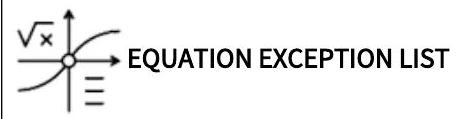
\includegraphics[max width=\textwidth, center]{2024_04_10_3ba0134d765492715516g-2}\\
$J B=(n / 6)\left[S^{2}+\left(K^{2} / 4\right)\right]$

where $J B$ is the Jarque-Bera test statistic, $n$ is the number of observations, $S$ is the skewness of the sample, and $K$ is the excess kurtosis of the sample.

Both the sample skewness and the kurtosis are computed as detailed in the previous sections. The null hypothesis is that the underlying distribution is normal and that $J B$ is equal to zero (since the skewness and excess kurtosis of the normal distribution are both zero).

While the Jarque-Bera test statistic is relatively easy to compute given the skewness and kurtosis, its interpretation is a little more complicated. Notice that $S$ and $K$ in the formula for the Jarque-Bera test statistic are both squared. Thus, the Jarque-Bera test will always be nonnegative. If the test did not square $S$ and $K$, a negative skewness would offset a positive excess kurtosis, which would wrongly suggest normality. As a sample exhibits more of the tendencies of a normal distribution (less skewness and less excess kurtosis), the Jarque-Bera test statistic will tend to be closer to zero (holding $n$ constant). Thus, the Jarque-Bera test for normality is whether the test statistic is large enough to reject the null hypothesis of normality. The Jarque-Bera test is more powerful when the number of observations is larger. If the underlying distribution is normal, the value of $J B$ generated from a sample will exceed zero with the known magnitudes and probabilities given by the chisquared distribution (with two degrees of freedom). Also, if the underlying distribution is normal, the size of the Jarque-Bera test statistic will tend to be small, since a sample drawn from a normal distribution will tend to have a low skewness and low excess kurtosis. The higher the $J B$ statistic, the less likely it is that the distribution is normal. The probability that the Jarque-Bera test statistic will exceed particular values can be found from a chi-squared distribution table, shown here with the required two degrees of freedom. These critical values for the Jarque-Bera test are formed through simulations.

\begin{center}
\begin{tabular}{|llllll|}
\hline
Confidence interval & 0.90 & 0.95 & 0.975 & 0.99 & 0.999 \\
Critical value & 4.61 & 5.99 & 7.38 & 9.21 & 13.82 \\
\hline
\end{tabular}
\end{center}

The analyst should perform the Jarque-Bera test in these four steps:

\begin{enumerate}
  \item Select a confidence interval (e.g., $90 \%, 95 \%, 97.5 \%, 99 \%$, or $99.9 \%$ ).

  \item Locate the corresponding critical value (e.g., 5.99 for $95 \%$ confidence).

  \item Compute the $J B$ statistic (using Equation 1 and the sample skewness and excess kurtosis).

  \item Compare the $J B$ statistic to the critical value.

\end{enumerate}

If the $J B$ statistic exceeds the critical value, then the null hypothesis of normality is rejected using the stated level of confidence. If the $J B$ statistic is less than the critical value, then the null hypothesis is not rejected, and the underlying distribution is assumed to be normal. The interpretation of this type of hypothesis test and the level of statistical confidence is actually quite complex and is discussed in detail in the Alpha, Beta, and Hypothesis Testing session.

\section*{An Example of the Jarque-Bera Test}
Assume that the sample skewness and excess kurtosis are computed as -0.577 and -0.042 , respectively. The sample size, $n$, is 40 . The Jarque-Bera test statistic is therefore given by:

$$
\begin{gathered}
J B=(n / 6)\left[S^{2}+\left(K^{2} / 4\right)\right] \\
J B=2.222
\end{gathered}
$$

Using a statistical confidence of $95 \%$, the critical value for the test is 5.99 . Since the Jarque-Bera test statistic, 2.222, is less than 5.99, we cannot reject the null hypothesis of normality.


\end{document}